\documentclass[12pt,a4paper]{article}
\usepackage{apacite}
\usepackage{graphicx}
\usepackage{amsmath}
\usepackage{natbib}
\usepackage{geometry}
\usepackage{setspace}
\usepackage{enumitem}
\usepackage{hyperref}
\usepackage{lipsum} % For placeholder text, remove it for actual content

% Page setup
\geometry{margin=1in}
\setstretch{1.5}
\setlength{\parindent}{0pt}
\setlength{\parskip}{1em}


% Title Page
\title{A Scalability Study of SHAP and TreeSHAP in Credit Scoring Applications}
\author{Group Members: \\
\textbf{Chan Jun Kit (1231302583)} \\
\textbf{Khan Shayan (1231301827)} \\
\textbf{Muhammad Ameer Rafiqi Bin Mohamad Shahizam (1211106255)} \\
\textbf{Marcus Chin Wei Hern (1211107284)} \\
\\
\textbf{Course:} Research Methodologies for Computer Science \\
Assignment 2 - Research Proposal \\
\textbf{Date of Submission:} September 25, 2024}
\date{}

\begin{document}

\maketitle
\newpage

% Executive Summary-----------------------------------------------------------
\section*{Executive Summary}
The rise of AI in credit scoring has significantly improved predictive accuracy but introduced challenges related to transparency and fairness, largely due to the "black box" nature of many AI models. Explainable AI (XAI) techniques, such as SHapley Additive exPlanations (SHAP), aim to address these challenges by providing insights into model decision-making processes. However, SHAP's high computational complexity and scalability limitations make its application in large-scale financial systems difficult.

This research investigates SHAP’s scalability in tree-based ensemble models, specifically Extreme Gradient Boosting (XGBoost), and explores methods to enhance its efficiency. The study focuses on two primary objectives: quantifying how SHAP’s scalability degrades with increasing prediction instances and identifying strategies, such as feature selection and TreeSHAP, that may improve scalability.

The methodology includes training two XGBoost models—one with full features and one with Chi-Square-selected features—using a large Lending Club dataset of 2.3 million loan applications. SHAP and TreeSHAP will be applied to both models, and the time complexity and explanation generation rates will be compared to assess scalability.

The outcomes will offer quantitative insights into SHAP's efficiency with large datasets and identify strategies to improve its scalability, which will be beneficial for enhancing transparency in AI-driven credit scoring.
\hfill
\\ \\
\textbf{Keywords:} Explainable AI (XAI), SHapley Additive exPlanations (SHAP), Scalability, Credit Scoring \\
\newpage

% Table of Contents---------------------------------------------------------
\tableofcontents
\newpage

% 1. Introduction------------------------------------------------------------
\section{Introduction}
\vspace{-1em}
The rise of artificial intelligence (AI) has revolutionised the financial industry, particularly in credit scoring, where machine learning models have significantly improved the accuracy of credit risk assessments. However, the "black box" nature of many AI models poses challenges related to transparency, fairness, and trust, especially in high-stakes decision-making processes such as loan approvals. As financial institutions increasingly adopt these advanced models, the need for explainable AI (XAI) techniques has become critical to ensure that credit-scoring decisions are understandable, transparent, and compliant with regulatory standards.

Among the various XAI methods, SHapley Additive exPlanations (SHAP) have gained attention for their ability to provide detailed, instance-level explanations of model predictions. Despite its effectiveness, SHAP often faces scalability issues, particularly when applied to tree-based ensemble models with large datasets. This research proposal aims to explore how the scalability of SHAP degrades with increasing data volume and investigates potential strategies, such as feature selection methods and optimised versions of SHAP (TreeSHAP), to improve its efficiency in credit scoring applications.





% 2. Problem statement-----------------------------------------------------
\section{Problem Statement}
\vspace{-1em}
In the quest to make robust but opaque credit-scoring models explainable and compliant, Explainable AI (XAI) techniques are applied to them. 
However, these techniques face several challenges:
\begin{enumerate}
    \item \textbf{Computational Complexity:} Many well-known XAI techniques, such as SHAP and LIME, are flagged for their computational complexity. SHAP, for instance, has an exponential time complexity \citep{misheva2021explainable}. Such a characteristic makes the XAI techniques challenging to scale as the volume of data grows and would not be viable in real-world settings where decisions and explanations are expected to be made swiftly.
    \item \textbf{Perturbation Process:} Perturbation is a critical process in many XAI techniques, whereby the XAI generates multiple slightly altered versions of a particular input to observe how the prediction changes and provide actionable explanations. In addition to the XAI techniques’ inherent computational complexity, this further inhibits their scalability.
\end{enumerate}

Although many papers acknowledge the difficulty of scaling XAI techniques \citep{marques2022delivering}, few focus on how to tackle the issue. There is also a lack of quantitative data on how specific XAI techniques are more time-efficient than others.
The scope of this research will be limited by only considering the scalability of SHAP on a tree-based, ensemble machine-learning model, specifically Extreme Gradient Boosting (XGBoost). 
This paper will explore strategies such as reducing the number of features (also known as dimensionality), employing the optimised version (TreeSHAP), or both to improve SHAP's scalability with a growing volume of requests. Equally important, this paper aims to quantify the effectiveness of the strategies in aiding scalability.




% 3. Research Questions, Hypotheses and Objectives----------------------------
\section{Research Questions, Hypotheses and Objectives}
\vspace{-1em}
\textbf{Research Questions:}\\
\vspace{-3em}
\begin{enumerate}
    \item How does the scalability of SHapley Additive exPlanations (SHAP) degrade as the volume of incoming prediction instances increases in a tree-based, ensemble machine learning model?
    \item How well can a feature-selection method or the optimised version of SHAP or both improve the scalability of SHAP in a tree-based, ensemble machine learning model?
\end{enumerate}

\textbf{Hypothesis:}\\
\vspace{-3em}
\begin{enumerate}
    \item The scalability of SHAP degrades exponentially as the volume of the incoming prediction instances increases in a tree-based, ensemble machine learning model.
    \item With a feature-selection method or the optimised version of SHAP or both, SHAP can handle more prediction instances before it reaches its practical capacity. 
\end{enumerate}

\textbf{Objectives:}\\
\vspace{-3em}
\begin{enumerate}
    \item To quantify how the scalability of SHAP degrades exponentially as the volume of the incoming prediction instances increases in a tree-based, ensemble machine learning model.
    \item To explore and quantify how a feature-selection method, or the optimised version of SHAP or both, can improve the scalability of SHAP in a tree-based, ensemble machine learning model.
\end{enumerate}





% 4. Literature Review--------------------------------------------------------
\section{Literature Review}
\vspace{-1em}
The literature review highlights the increasing role of AI in credit scoring, showing how AI models like random forests, neural networks, and XGBoost significantly enhance predictive accuracy compared to traditional statistical methods. However, these models’ "black box" nature poses challenges related to transparency, fairness, and ethical considerations in financial decision-making.

To address these challenges, researchers have explored various XAI techniques, such as SHAP, LIME, GIRP + SHAP, Anchors, and ProtoDash, aiming to improve the interpretability of AI-driven credit scoring models \citep{demajo2020explainable}. These techniques provide both local and global explanations, helping stakeholders understand and trust AI-based decisions in credit scoring. While XAI methods offer opportunities for enhanced transparency, they face computational complexity and scalability issues, particularly when dealing with large datasets \cite{demajo2020explainable}. SHAP, for instance, is particularly limited by exponential time complexity with large datasets \citep{misheva2021explainable}.

\textbf{Gaps Identified:}\\
\vspace{-3em}
\begin{enumerate}
    \item \textbf{Scalability of XAI Techniques:} The existing literature rarely examines the scalability of XAI methods like SHAP in handling large, real-world datasets, particularly in ensemble machine learning models.
    \item \textbf{Bias Mitigation and Real-World Application}: Researchers discuss how XAI can identify bias but often overlook how to use XAI to mitigate biases actively during decision-making processes. Additionally, the literature lacks real-world case studies demonstrating XAI's implementation in financial institutions.
\end{enumerate}

\textbf{Trends:}\\
\vspace{-3em}
\begin{enumerate}
    \item Use of Real-Time and Evolving Data: Researchers increasingly use dynamic, real-world datasets from institutions like Lending Club, showing the importance of adapting models to current borrower behaviour and regulatory changes \citep{misheva2021explainable} \citep{demajo2020explainable}.
    \item Complementary Use of Multiple XAI Techniques: We observe a trend where researchers combine multiple XAI techniques to enhance both interpretability and accuracy in credit scoring models, addressing the diverse needs of stakeholders \citep{demajo2020explainable}.
\end{enumerate}

\textbf{Implications for Future Research:}\\
\vspace{-3em}
\begin{enumerate}
    \item Real-World Implementation and Case Studies: Future studies should focus on empirical case studies of XAI implementation in financial institutions, examining practical impacts on customer trust, bias reduction, and regulatory compliance \citep{sadok2022artificial}.
    \item Scalability and Efficiency of XAI Techniques: Researchers should explore how feature-selection methods or optimised versions of SHAP can enhance scalability in large datasets, particularly in ensemble models \citep{TRIVEDI2020101413}.
\end{enumerate}



% 5. Research Methodology-----------------------------------------------------
\section{Research Methodology}
\vspace{-1em}
This project consists of the following main components:\\
\vspace{-3em}
\begin{enumerate}[label=\Alph*., itemsep=0.1em]
    \item Data gathering and preprocessing
    \item Model training
    \item Testing XAI methods
    \item Data collection and analysis
    \item Data visualisation
\end{enumerate}
\textbf{PART A – DATA COLLECTION AND PREPROCESSING}\\
We will be using the Lending Club (LC) Dataset, which includes around 2.3 million loan applications with 145 features of different types \citep{demajo2020explainable}. Firstly, the data is cleaned by handling any special values, encoding categorical variables into numerical formats and eliminating noisy data and outliers. Next, an analysis of the correlation matrix will be performed on the dataset to remove redundant features. Finally, the data will be split with an 80:20 ratio using stratification into training and testing sets.

\textbf{PART B – MODEL TRAINING}\\
Two different machine learning models will be trained using Extreme Gradient Boosting (XGBoost) as the base mode:\\
\vspace{-3em}
\begin{enumerate}
    \item Full Feature XGBoost: This model will use all the features from the dataset without applying any feature selection techniques.
    \item Chi-Square Feature Selection XGBoost: We chose the Chi-Square Test as our feature selection technique due to its performance in \citep{TRIVEDI2020101413}. The test ranks features based on relevance, and only the top-ranked features are selected for model training. This model will be referred to as the pruned XGBoost.
\end{enumerate}
\vspace{-1em}
Both models will be trained on the pre-processed LC Dataset to ensure comparability using the same hyperparameters. Cross-validation will ensure robustness in model performance.

\textbf{PART C – TESTING THE SCALABILITY OF SHAP}\\
SHAP and TreeSHAP will generate an explanation for the decisions made by the models. TreeSHAP is an optimised version of SHAP designed specifically for tree-based models like XGBoost \citep{muschalik2024beyond}. The goal is to evaluate the time taken for SHAP/TreeSHAP to generate explanations under varying conditions. Four scenarios will be tested:
\vspace{-1em}
\begin{enumerate}
    \item SHAP + Full Feature XGBoost
    \item SHAP + Pruned XGBoost
    \item TreeSHAP + Full Feature XGBoost
    \item TreeSHAP + Pruned XGBoost
\end{enumerate}
\vspace{-1em}
In each scenario, the selected model will be instructed to generate predictions at an increasing rate of requests per minute. The time taken to generate explanations will be recorded for each minute.

\textbf{PART D – DATA ANALYSIS}\\
The primary metrics that this paper will analyse are:
\vspace{-1em}
\begin{enumerate}
    \item \textbf{Time complexity:} The time taken to generate explanations at each rate of incoming predictions. This will be measured for each scenario.
    \item \textbf{Scalability:} The system’s ability to keep up with explanation generation will be evaluated. The point at which explanation time exceeds acceptable limits will indicate the scalability threshold.
    \item \textbf{Feature Selection Impact:} The difference in time between models with and without feature selection will be analysed to determine the impact of feature selection on scalability.
\end{enumerate}
	
\textbf{PART E – DATA VISUALISATION}\\
All collected data will be visualised to illustrate the time complexity and scalability of SHAP and TreeSHAP. The visualisation will include:
\vspace{-1em}
\begin{enumerate}
    \item \textbf{Explanation Time vs. Request Rate:} The plot shows how explanation time changes as the number of incoming prediction instances per minute increases.
    \item \textbf{Comparison of Methods:} Side-by-side comparisons of the four different combinations of models to highlight the effects of feature selection and optimisation.
    \item \textbf{Scalability Threshold:} Identifying the point at which each combination becomes computationally expensive or impractical for real-time applications.
\end{enumerate}
	
\newpage

% 6. Research Activities and Milestones---------------------------------------
\section{Research Activities and Milestones}
\vspace{-1em}
\textbf{Activity Flowchart:} 
\begin{figure} [htbp]
    \centering
    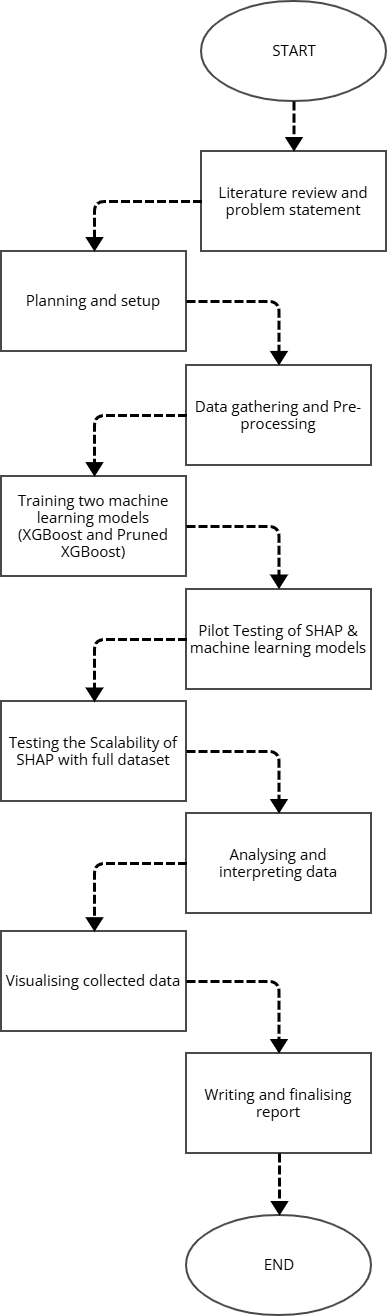
\includegraphics[width=0.3\linewidth]{Activity Flowchart.png}
    \caption{Activity Flowchart}
    \label{Activity flowchart}
\end{figure}

\newpage

\textbf{Research Activities:}\\
\vspace{-2em}
\begin{table}[h]
    \centering
    \begin{tabular}{| l | c | c |}
    \hline
    \textbf{Activity} & \textbf{Start Date} & \textbf{End Date} \\
    \hline
    Planning and Setup & 01/01/2025 & 28/02/2025 \\
    \hline
    Data Gathering and Pre-processing & 01/03/2025 & 30/03/2025 \\
    \hline
    Model Training & 01/04/2025 & 16/05/2025 \\
    \hline
    Pilot Testing & 17/05/2025 & 16/06/2025 \\
    \hline
    Testing SHAP with Full Dataset & 17/06/2025 & 17/08/2025 \\
    \hline
    Data Analysis and Integration & 18/08/2025 & 30/09/2025 \\
    \hline
    Report Writing and Publication & 01/10/2025 & 31/12/2025 \\
    \hline
    \end{tabular}
    \caption{Research Activities}
    \label{Research Activities}
\end{table}


\textbf{Milestone and Dates:} 
\begin{table}[h]
    \centering
    \begin{tabular}{| p{8cm} | c | p{5cm} |}
    \hline
    \textbf{Activity} & \textbf{Date} & \textbf{Cumulative Completion Percentage (\%)} \\
    \hline
    Completion of Planning and Setup & 28/02/2025 & 10 \\
    \hline
    Completion of data gathering and pre-processing & 30/03/2025 & 20 \\
    \hline
    Completion of model training & 16/05/2025 & 35 \\
    \hline
    Completion of pilot testing & 16/06/2025 & 45 \\
    \hline
    Completion of the full experiment & 17/08/2025 & 60 \\
    \hline
    Completion of data analysis and visualisations & 30/09/2025 & 75 \\
    \hline
    Completion of report and publication & 31/12/2025 & 100 \\
    \hline
    \end{tabular}
    \caption{Research Activities}
    \label{Research Activities}
\end{table}

\newpage

\textbf{Gantt Chart with Research Activities and Milestones:}
\begin{figure}[h]
    \centering
    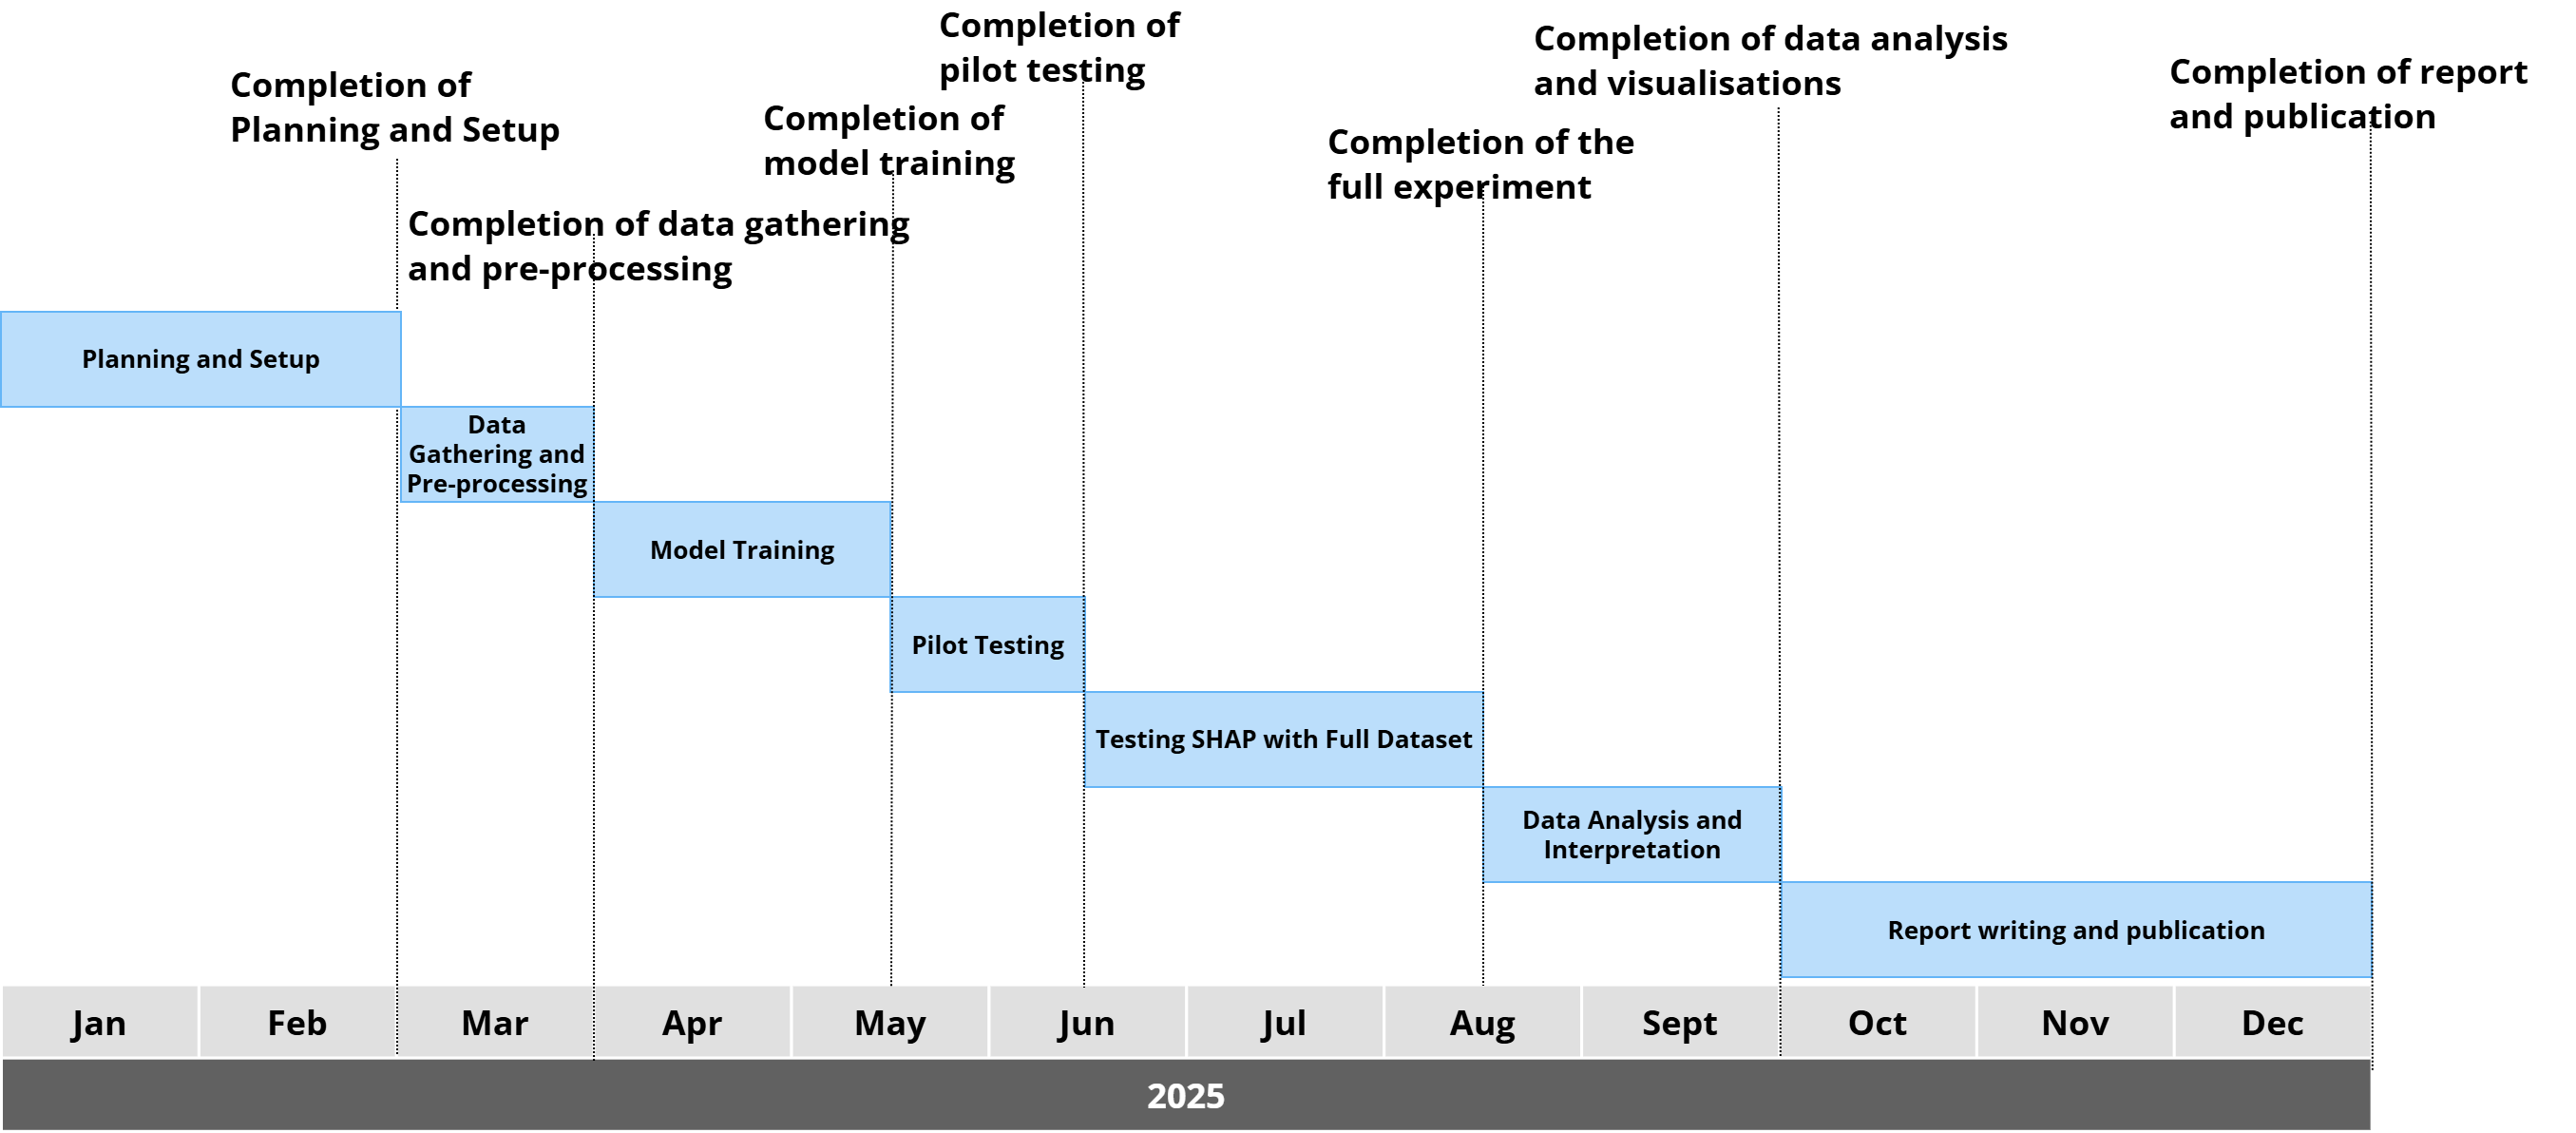
\includegraphics[width=1\linewidth]{Gantt Chart.png}
    \caption{Gantt Chart with Research Activities and Milestones}
    \label{fig:enter-label}
\end{figure}


% 7. Expected Results and Impact----------------------------------------------
\section{Expected Results and Impact}
\vspace{-1em}
\begin{enumerate}
    \item \textbf{Novel Theories/Findings:}
    \begin{itemize}
        \item Provide quantitative insights into SHAP’s scalability in tree-based ensemble models, filling a gap in current literature.
        \item Identify effective strategies (feature selection, TreeSHAP) to improve SHAP’s efficiency in handling high-volume datasets.
        \item Offer solid, quantified data to guide future researchers in XAI scalability studies.
    \end{itemize}

    \item \textbf{Impact on Society, Nation, and Economy:}
    \begin{itemize}
        \item Enhance the explainability of AI-driven credit decisions, building trust among consumers and regulators.
        \item Support financial institutions in meeting transparency requirements, ensuring fair and ethical AI deployment.
        \item Improve credit decision accuracy and speed, lowering operational costs and promoting wider access to credit, aiding underserved communities.
        \item Contribute scalable XAI methods applicable beyond finance, benefiting sectors like healthcare, insurance, and legal systems.
    \end{itemize}
\end{enumerate}




% References--------------------------------------------------------
\newpage
\bibliographystyle{apacite} 
\bibliography{MyBib} 


% Appendices
\appendix
\section{Appendix A: Member Contributions}

\vspace{-10pt}

\begin{table}[h]
    \centering
    \begin{tabular}{|c|c|c|}
        \hline
        \textbf{Name} & \textbf{Student ID} & \textbf{Contribution (\%)} \\ \hline
        Chan Jun Kit  & 1231302583 & 25   \\ \hline
        Khan Shayan   & 1231301827 & 25   \\ \hline
        Muhammad Ameer Rafiqi Bin Mohamad Shahizam & 1211106255 & 25  \\ \hline
        Marcus Chin Wei Hern & 1211107284 & 25   \\ \hline
        \multicolumn{2}{|r|}{\textbf{Total}} & 100 \\ \hline
    \end{tabular}
\end{table}

\end{document}